\textbf{Name:} Patrick L. Harvey \\

\medskip

\textbf{Conspirators:} \href{https://doi.org/10.1140/epjds/s13688-021-00260-3}{Ryan J. Gallagher, Morgan R. Frank, Lewis Mitchell, Aaron J. Schwartz, Andrew J. Reagan, Christopher M. Danforth, and Peter Sheridan Dodds}

\href{https://www.overleaf.com/read/jwptqkrxjbkr}{Self-referential location} for this document.\\
\href{https://github.com/P-Harvey/csys303_assignments/tree/main/plharvey_19}{Repository for code that may not be guaranteed to be 100$\%$ good to go.}
\medskip
\medskip

\hrule

\medskip


\begin{enumerate}

\item
  \label{q1}Surface area of allometrically growing \sout{Love}Minecraftian organisms:

  Let's consider animals as parallelepipeds (e.g., the well known box cow),
  with dimensions $L_1$, $L_2$, and $L_3$
  and volume $V = L_1 \times L_2 \times L_3$.

  Let's assume 
  length $L_{i}$
  scales with volume as 
  $
  L_{i}
  =
  c_{i}^{-1}
  V^{\gamma_{i}}
  $
  where the exponents satisfy
  $
  \gamma_{1}
  +
  \gamma_{2}
  +
  \gamma_{3}
  =
  1
  $
  and the $c_{i}$ are prefactors such that
  $c_1 \times c_2 \times c_3 = 1$.
  Let's also arrange our organisms so that
  $
  \gamma_{1}
  \ge
  \gamma_{2}
  \ge
  \gamma_{3}
  $.

  \begin{enumerate}
  \item 
    Show that the scalings 
    $
    L_{i}
    =
    c_{i}^{-1} V^{\gamma_{i}}
    $
    mean that indeed 
    $
    L_{1}
    \times
    L_{2}
    \times
    L_{3}
    =
    V
    $.
  \item 
    Write down the $\gamma_{i}$ corresponding to isometric scaling.
  \item 
    Calculate the surface area $S$ of our imaginary blockular beings for general
    allometric scaling of the sides.
  \item 
    Show how $S$ behaves as $V$ becomes large (i.e., which term(s) dominate).
  \item 
    Which sets of $\gamma_{i}$ give the fastest and slowest possible
    scaling of $S$ as a function of $V$?
  \end{enumerate}

%%  Note: surface area is a big deal for organisms and this calculation
%%  will matter later in PoCS Vol.\ 1 and/or PoCS Vol. 2 (CocoNuTs)

  Relevant tarot cards, for your consideration:
  
  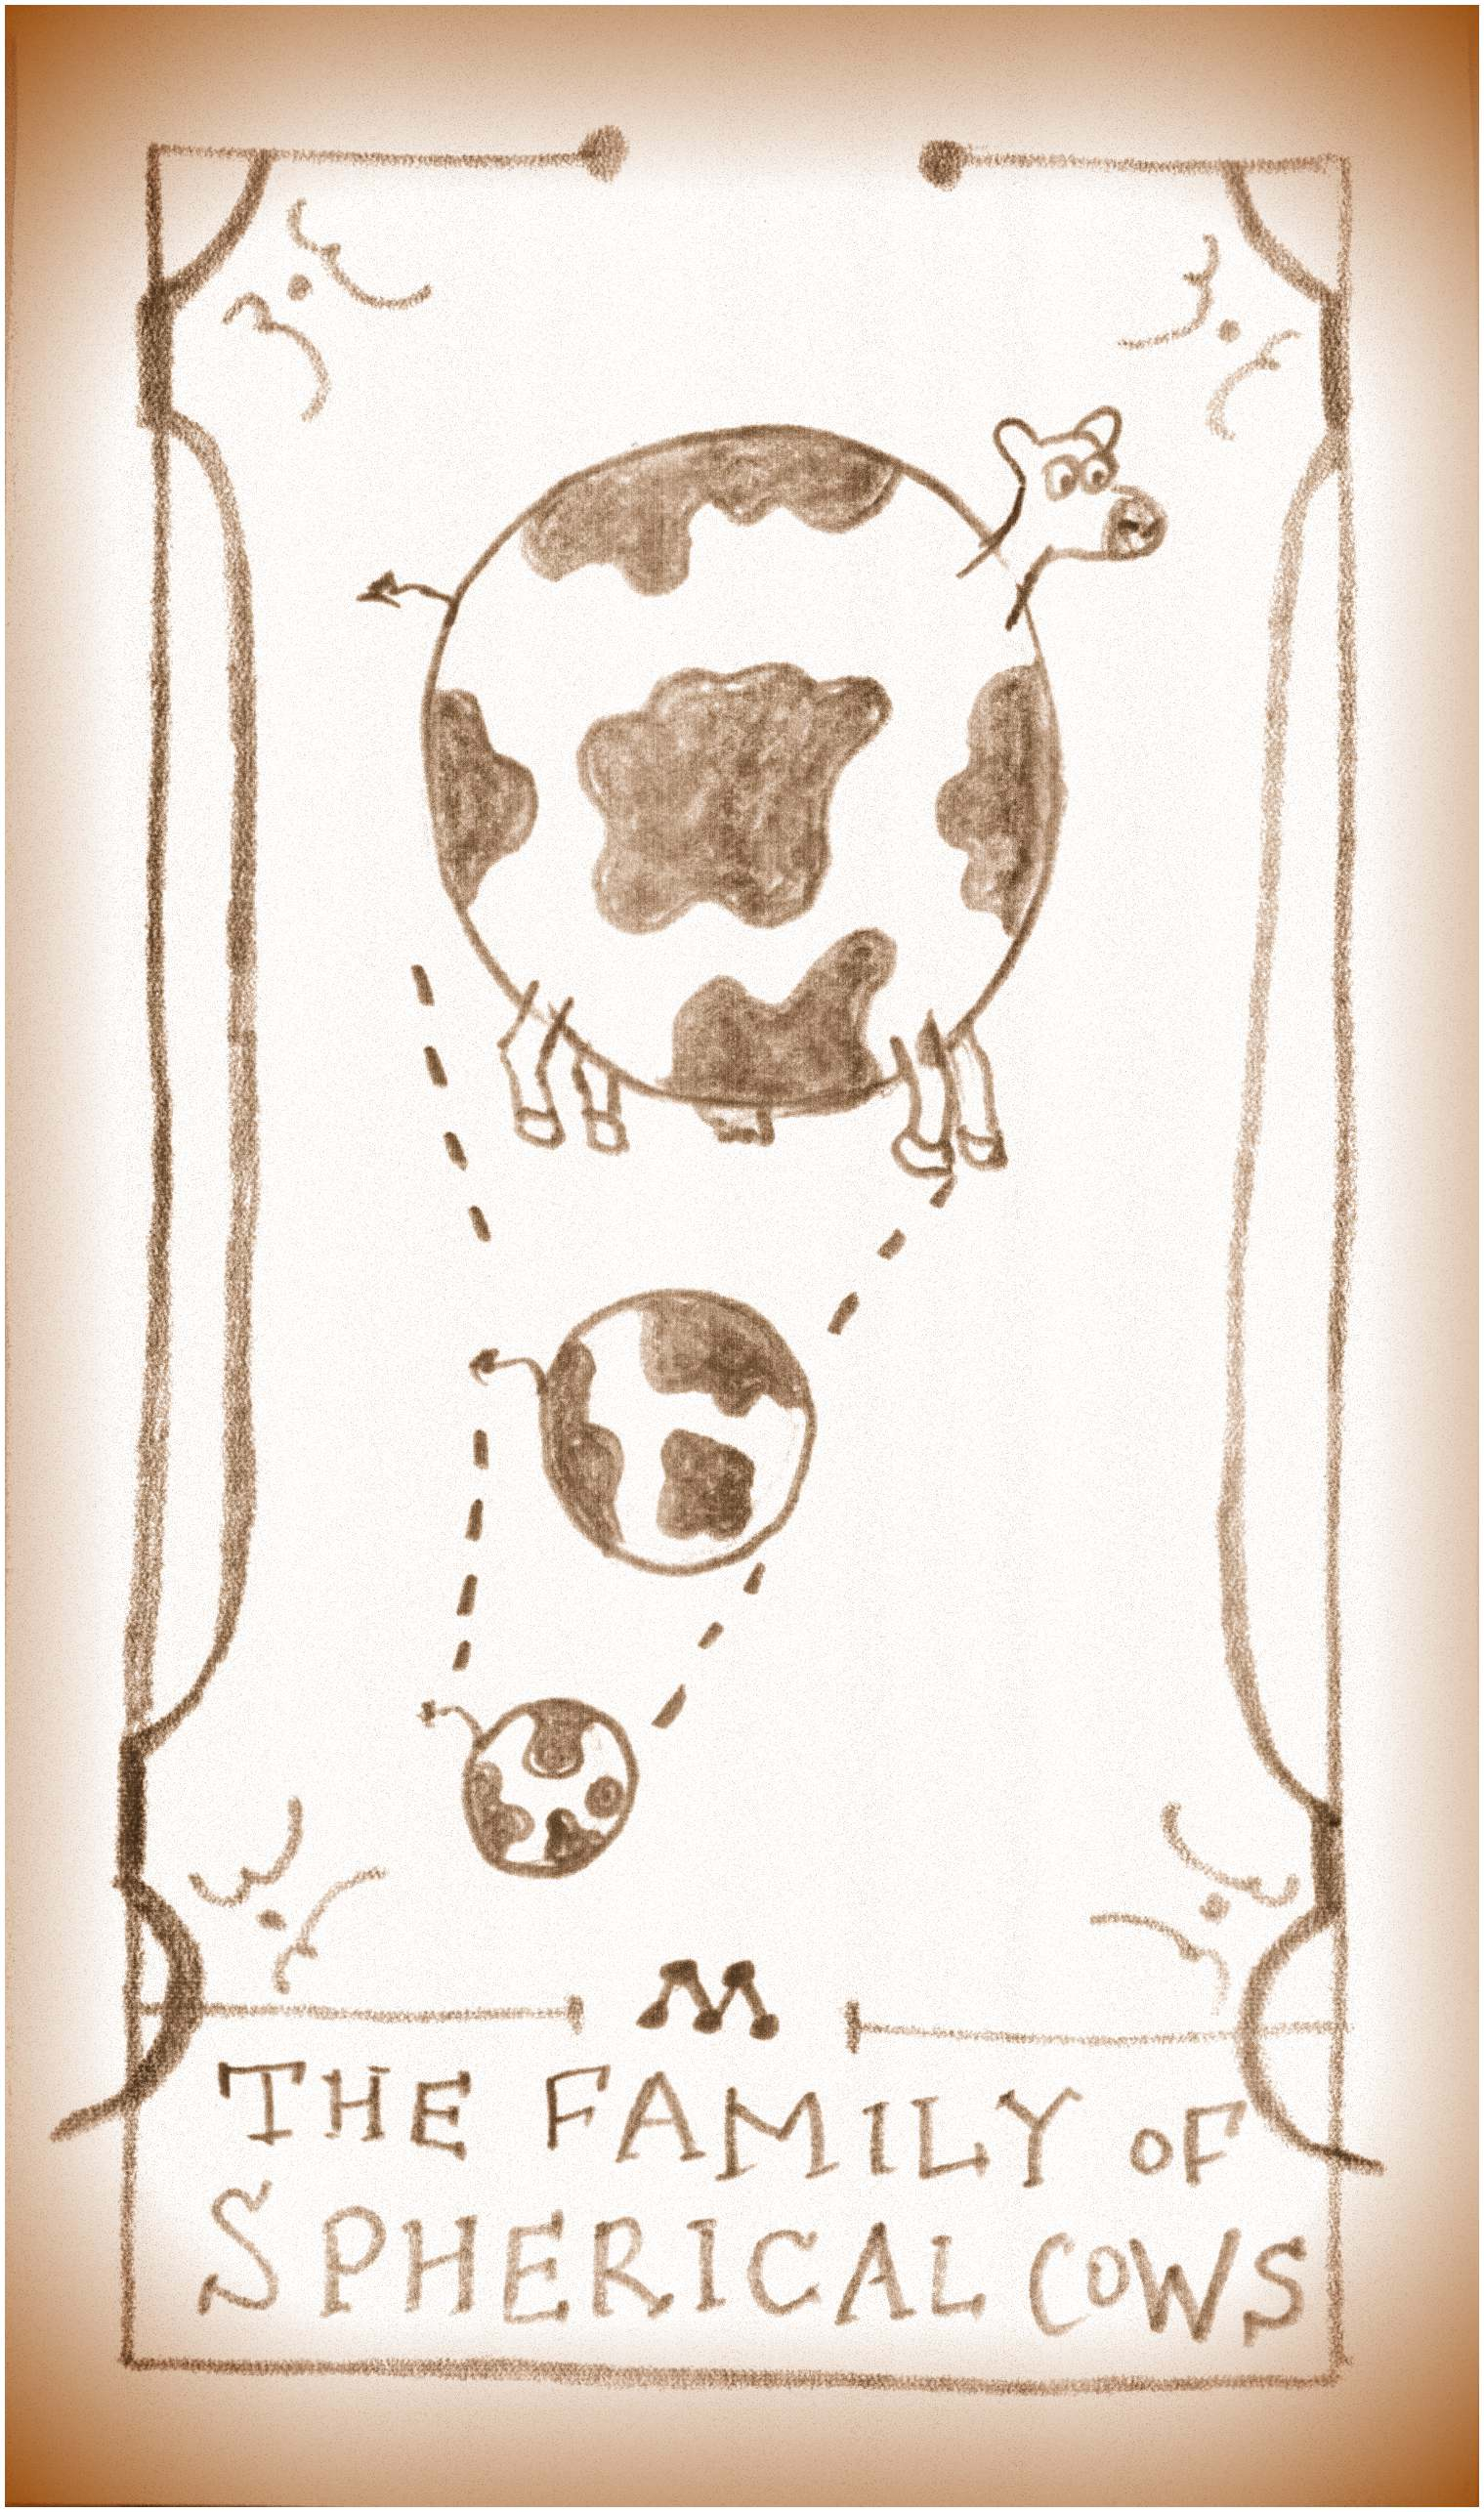
\includegraphics[width=0.30\textwidth]{tarot-card-scaling-spherical-cows.jpg}
  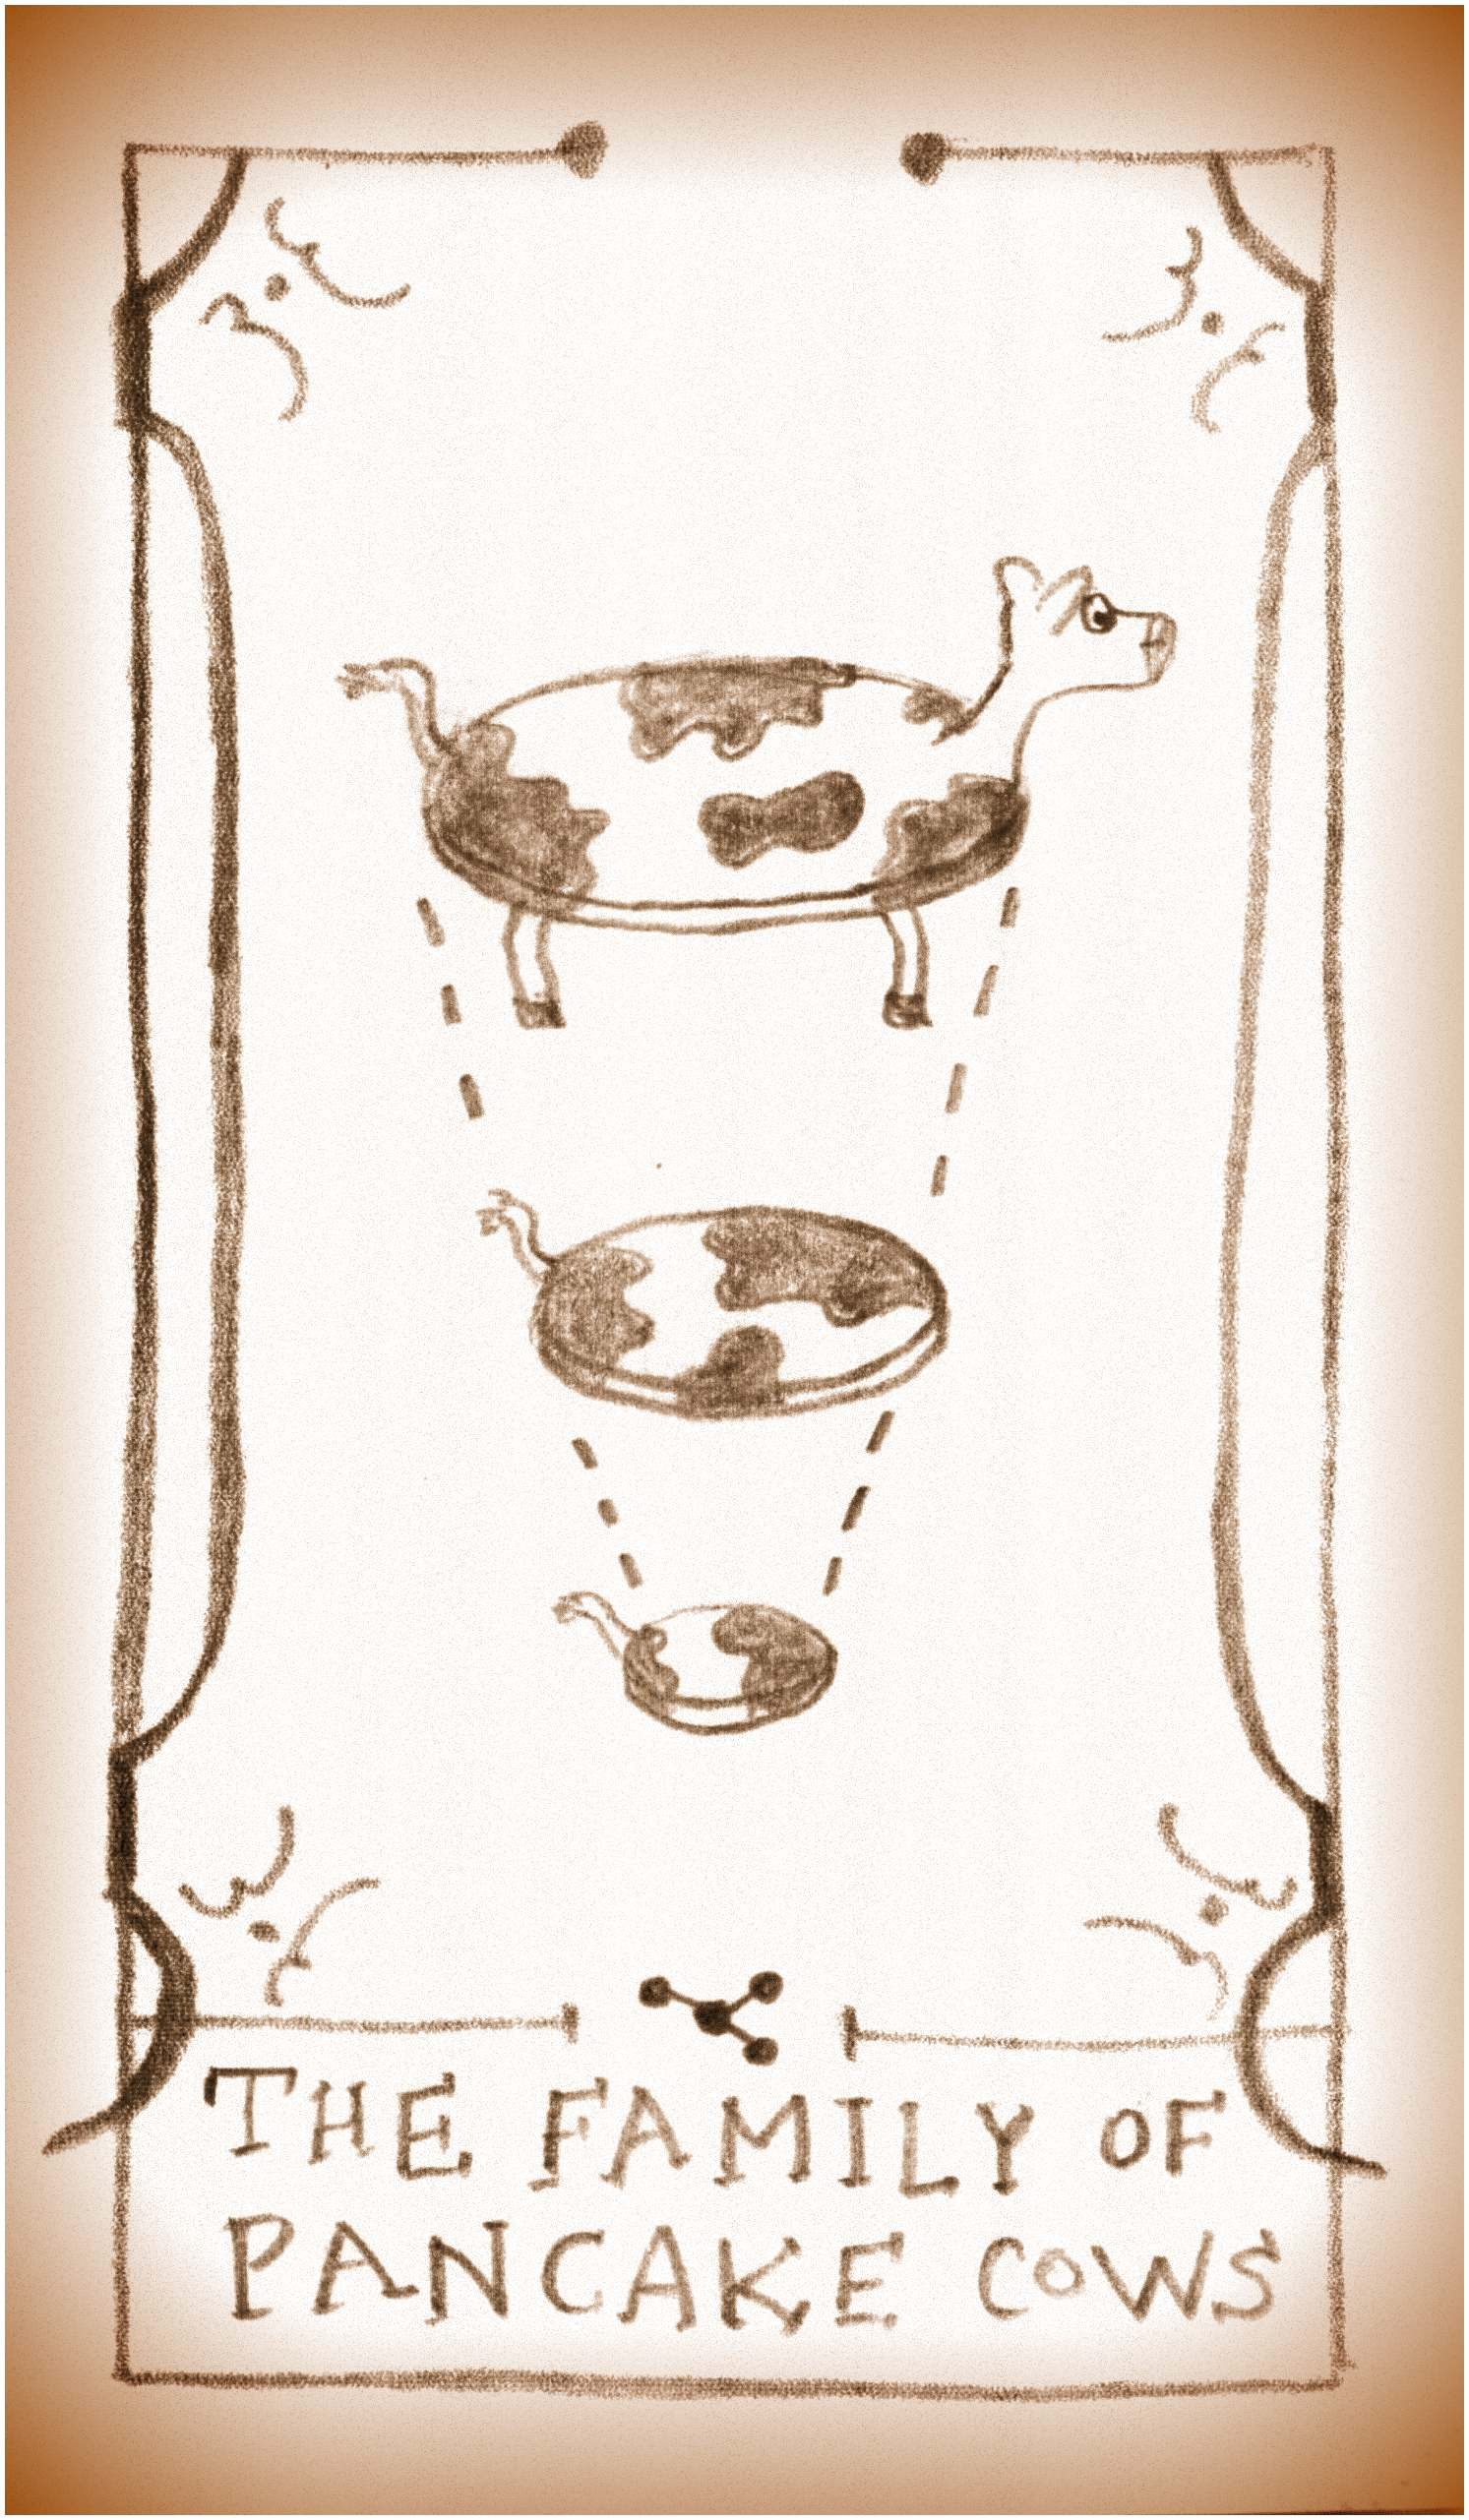
\includegraphics[width=0.30\textwidth]{tarot-card-scaling-pancake-cows.jpg}
  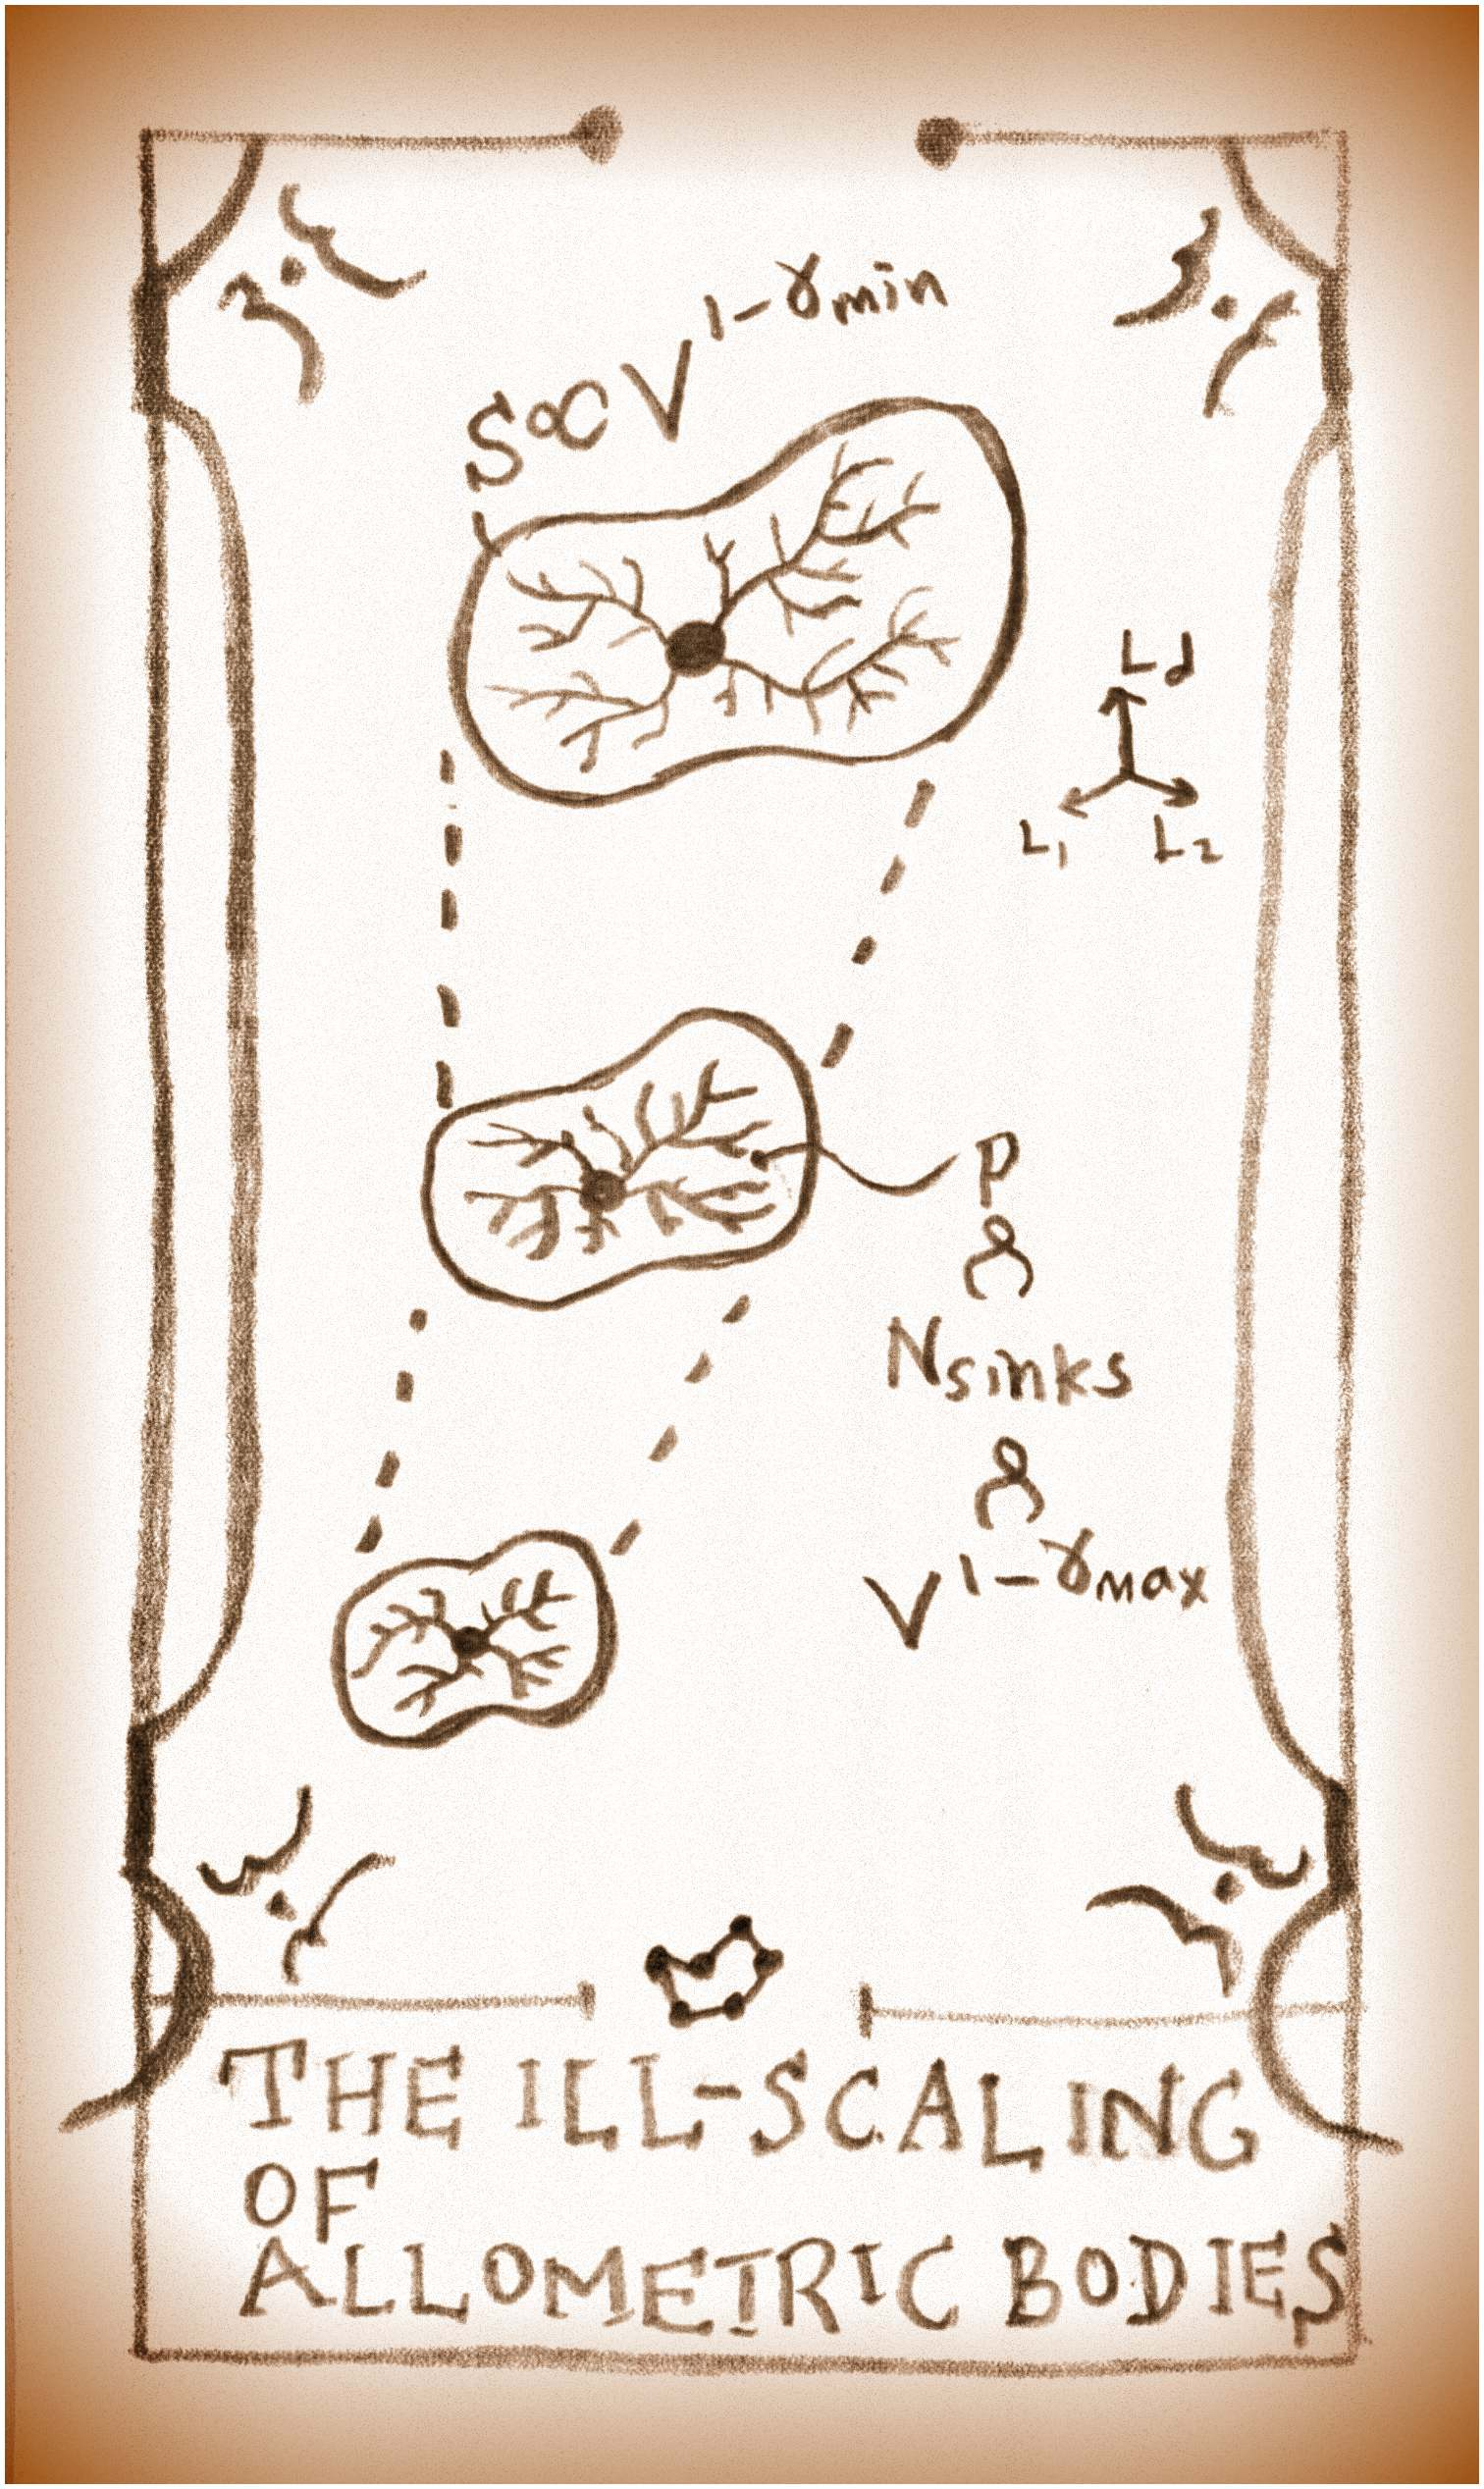
\includegraphics[width=0.30\textwidth]{tarot-card-ill-scaling-of-allometric-bodies.jpg}

  
   \solutionstart
   
(a) Given dimensions:\\
\begin{equation}
    V = L_1 \times
        L_2 \times
        L_3
        \label{ass_19::eq_1}
\end{equation}
Where:
\begin{equation}
   L_i = c_i^{-1}
         V^{\gamma_i}
         \label{ass_19::eq_2}
\end{equation}
\begin{equation}
   1 =  \gamma_1 + 
        \gamma_2 + 
        \gamma_3
        \label{ass_19::eq_3}
\end{equation}
\begin{equation}
   1 = c_1 \times
       c_2 \times
       c_3
       \label{ass_19::eq_4}
\end{equation}
and
\begin{equation}
   \gamma_1 \geq \gamma_2 \geq \gamma_3 \label{ass_19::gammas}
\end{equation}
We want to show that $V = L_1 \times L_2 \times L_3$ is valid.

Let's start by rearranging equation (\ref{ass_19::eq_1}) such that:
\begin{align*}
   L_i = \frac{1}{c_i}
         V^{\gamma_i}
\end{align*}
Which allows us to show the proportional relationship between our being's volume and linear dimensions as:
\begin{equation}
   \frac{V^{\gamma_i}}{L_i} = c_i \label{ass_19::eq_5}
\end{equation}

From here we can substitute equation (\ref{ass_19::eq_5}) into (\ref{ass_19::eq_3}) to get:
\begin{align*}
   1 &= 
        \frac{V^{\gamma_1}}{L_1}
        \times
        \frac{V^{\gamma_2}}{L_2}
        \times
        \frac{V^{\gamma_3}}{L_3}\\
     &= \frac{V^{\gamma_1 +
                 \gamma_2 +
                 \gamma_3}}
             {L_1 \times
              L_2 \times
              L_3 \times}\\
    L_1 \times
    L_2 \times
    L_3 \times &= V^{\gamma_1 +
                 \gamma_2 +
                 \gamma_3}
\end{align*}

Using (\ref{ass_19::eq_2}) we see that:
\begin{align*}
   L_1 \times
   L_2 \times
   L_3 \times &= V^{1}\\
   L_1 \times
   L_2 \times
   L_3 \times &= V \\
   \Rightarrow
   V &= 
   L_1 \times
   L_2 \times
   L_3 \label{ass_19::q_1_a}
\end{align*}
Validating our parallelepiped's scaling relationship in Eq.(\ref{ass_19::eq_1}).\clearpage

(b): The answer to the question is $\gamma_i = \frac{1}{3}$. Let's unpack it.

\hypertarget{isometric}{We'll start by determining trying to figure out how $\gamma_i$ corresponds to isometric scaling of the parallelepiped}.

Rearranging (\ref{ass_19::eq_5}) we can proceed as follows:
\begin{align*}
   \frac{V^{\gamma_i}}{L_i} &= c_i\\
   \Rightarrow V^{\gamma_i} &= c_i L_i
\end{align*}

In other words, the parallelepiped's length is proportional to it's volume exponentiated:
\begin{align*}
   V^{\gamma_i} &\propto L_i\\
   \ln{(V^{\gamma_i})} &\propto
             \ln{(L_i)}\\
   \gamma_i \ln{(V)} &\propto
             \ln{(L_i)}\\
   \gamma_i &\propto
             \frac{\ln{(L_i)}}
             {\ln{(V)}}\\
\end{align*}

If we wanted to be specific:
\begin{align*}
   \gamma_i &= c_i
             \frac{\ln{(L_i)}}
             {\ln{(V)}} \label{ass_19::q_1_b}\\
\end{align*}

To get isometric scaling we would want $\gamma_i$ to exist such that we have a $3:1$ correspondence of $L$ with $V$ (since we can usually comprehend three dimensions well enough). The implication, given the setup, is either:
\begin{align*}
   \gamma_i &= \frac{1}{3}\\
   \gamma_1 &= \gamma_2 = \gamma_3\\
   \textnormal{if }
        L_1 &= L_2 = L_3\\
          V &= k {L^{3}}
\end{align*}

\hypertarget{allometric}{or}:
\begin{align*}
   \frac{1}{3} \geq &\gamma_3 \geq 0\\
   \frac{1}{2} \geq &\gamma_1, \gamma_2 \geq \frac{1}{3}\\
   \textnormal{giving }
          V^{\gamma_i} &= \prod_{i=1}^{3} \frac{1}{c_i} L_i\\
   \textnormal{where }
        L_1 &\geq L_2 \geq L_3\\
        \Rightarrow
        V &= k \prod_{i=1}^{3} {L_{i}^{1/\gamma_i}}\\
   \textnormal{letting } 
          k &= \frac{1}{c_1 \times c_2 \times c_3}
    \label{allometric}
\end{align*}
The "or" can lead to interesting scenarios.
Let's save it for future reference.

\clearpage
   
(c):

Now we want to know how the surface area of the parallelepiped's surface area ($S$) changes with respect to it's linear dimensions ($L_{i}$) under allometric (a.k.a power-law) scaling (e.g. $S = k L_{i}^{\alpha}$).

Let's start by thinking about this problem geometrically.
By definition,
the area of a flat-planed (two-dimensional) surface is equal to the product of it's basis (e.g. length $\times$ width).
Let's expand this to a three-dimensional space.
Now we can look at the relationship between surface area and linear measure such that $S = 6 L^2$.
That is,
we are combining some countable ($6$) number of surfaces together to enclose a space that we will call box-cow.
Let's also make an assumption that our box-cow is not missing any of its faces.

In other words,
a side ($\textnormal{Side}_{ij}$) would have surface area that behaves as $\textnormal{Side}_{ij} = S_{ij} = L_i \times L_{j}$.

Given what we know from Eq.(\ref{ass_19::eq_1}),
we also know that the total surface area of our \sout{square-cube} box-cow has a direct relationship with its volume.

Let's find out what that relationship has to be so we can get general allometric scaling.

Since we know that the volume is the (scalar triple) product of the three linear bases from (\ref{ass_19::eq_1}), 
and that $L_i=\sqrt[3]{V}$ (iff linear measures are equal), 
let's consider this as our input function which we will map to our desired output ($S$). 
Which should give us $S$ in terms of the product of our linear measures ($L_{i}$).
Looking at how this relationship scales when all things ($L_1, L_2, L_3$) are not created equal requires us to consider the non-redundant pairwise combinations as below:
$$
   S_{ij} = L_i \times L_j \textnormal{ given } i \neq j
$$

or:

$$
   S = 2
   \bigg(
   (L_1 \times L_2) +
   (L_1 \times L_3) +
   (L_2 \times L_3)
   \bigg)
$$

For isometric scaling, 
we would want proportional growth (e.g. a square-cube law...). 
That is, 
the surface area grows as the squared ratio of its two differing lengths (or support vectors), 
while the volume would increase as the cubed ratio of the same lengths.
This logic leads to:
\hyperlink{isometric}{
\begin{align*}
    L_1 &= L_2 = L_3 = 1\\
    L_1 + L_2 &= 2^0 + 2^0 \Rightarrow 2^1\\
    S &= 2^1 \times 2^1 \Rightarrow 2^2\\
    V &= 2^1 \times 2^1 \times 2^1 \Rightarrow 2^3
\end{align*}}
and so on for presumably higher dimensions.

The assumption here is that the linear measure omitted
(e.g. $L_3$)
is equal (redundant/collinear) with other linear measures.

Since we looking for allometry,
we're going to pick up at \hyperlink{allometric}{"or"}\\
\tiny
xor $\frac{dV}{dL} \neq 3$.
\normalsize

Given our assumptions that
$\gamma_1 \geq \gamma_2 \geq \gamma_3$
and $\gamma_1 + \gamma_2 +\gamma_3 = 1$
we may find that the smallest $\gamma$ of the bunch can cause a bit of disorder.
Let's consider some $\gamma_3 \neq \frac{1}{3}$:
\begin{align*}
    L_1 + L_2 + L_3 &= \sum_{i=1}^3 L_i\\
    S &= 
    2 \bigg(
    \sum_{i, j = 1}^{3} L_i \times L_j
    \bigg) \textnormal{ given }i \neq j
\end{align*}
Giving \sout{something like} a sum of pairwise squares for $S$,
which brings us back to our interesting $V$:
\begin{align*}
    V &= k \prod_{i=1}^{3} {L_{i}^{1/\gamma_i}}\\
    &\textnormal{expanding to}\cdots\\
    V &= k  \left( 
            {L_{1}^{1/\gamma_1}}
            \times
            {L_{2}^{1/\gamma_2}}
            \times
            {L_{3}^{1/\gamma_3}}
            \right)
\end{align*}
Clearly,
any situation where $\gamma_3 \leq \frac{1}{3}$ leads to something allometric.
So, given our setup, $\gamma_3$ and $L_3$ control the deviation from isometry.
Looking back at $S$, which is not dependent on exponentiation, we retain the triple product squared growth.
So as $V \to \textnormal{big, } S \to \textnormal{bigger}$.
Specifically:
$$
S = k V^{1-\alpha}
$$

\clearpage

(d): Enjoy some plots.\\
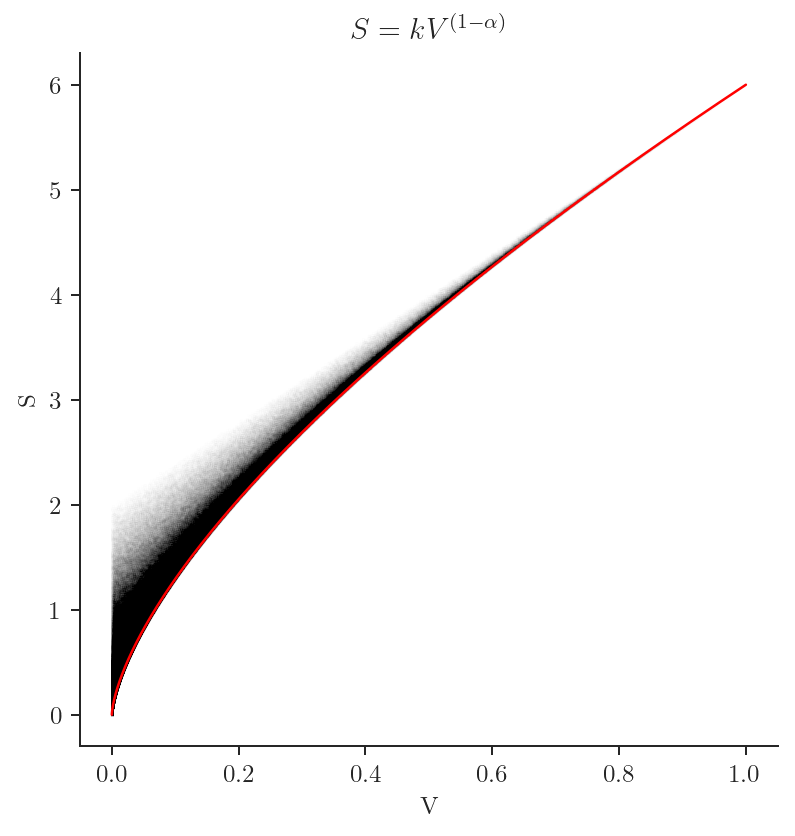
\includegraphics[width=0.45\textwidth]{figures/iso_alo.png}
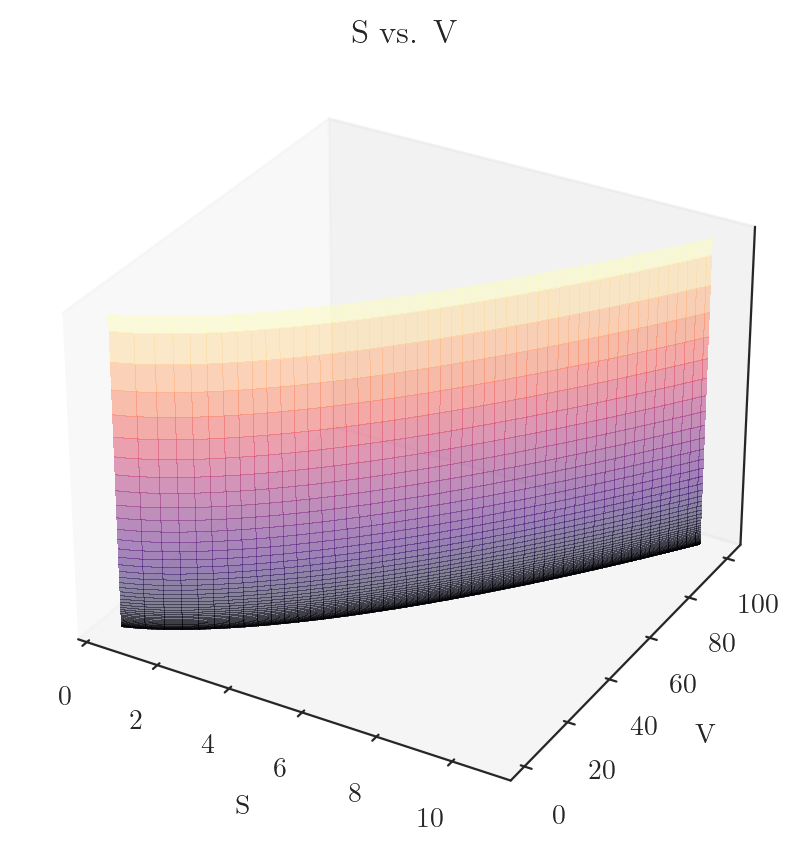
\includegraphics[width=0.45\textwidth]{figures/S_vs_V_3D.png}\\
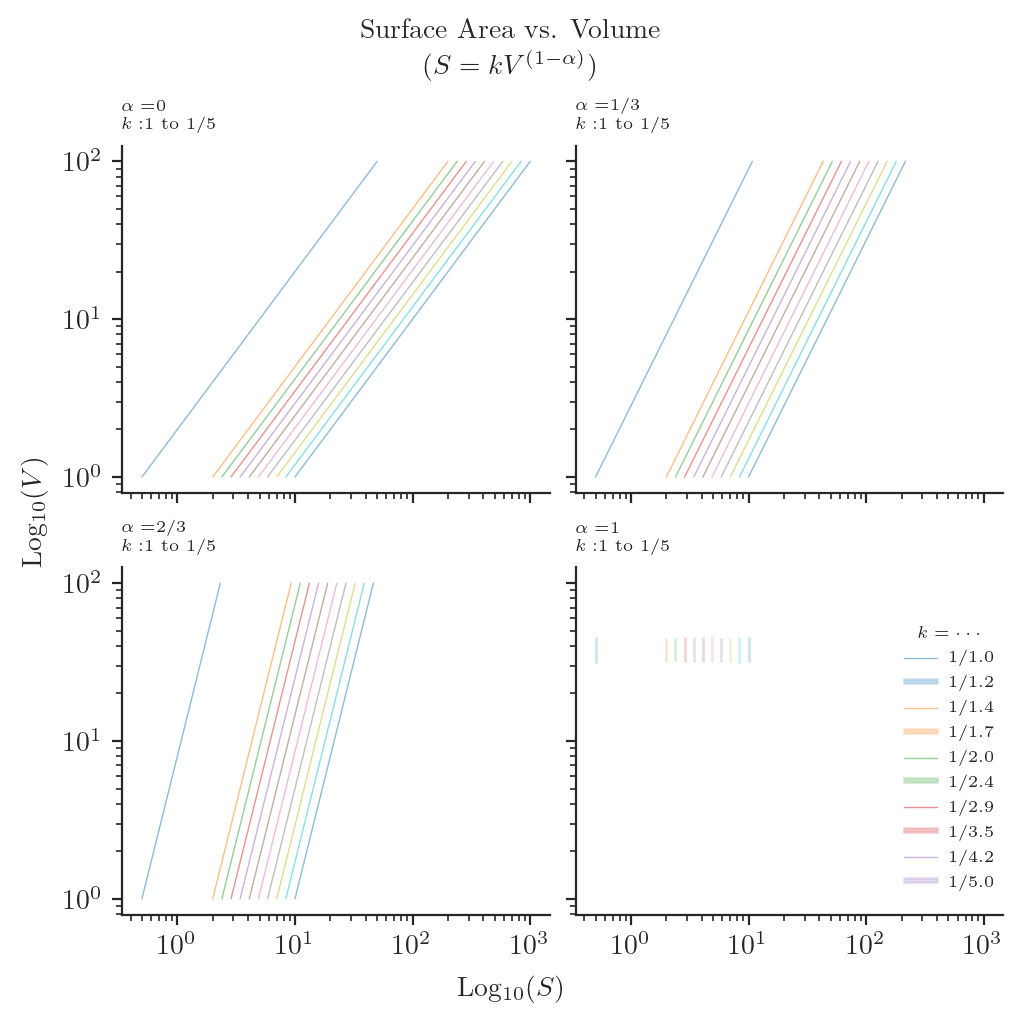
\includegraphics[width=0.8\textwidth]{figures/S_vs_V.png}\\
Top Left: Red is standardized isometric scaling, black is random allometric deviations from isometry.
Isometric scaling sets the lower bound for $S$ with respect to $V$.
That is, any deviation from proportional growth of side lengths leads to larger values of $S$ with respect to $V$.

(e):

For any \sout{non-isometric} general allometric scaling we will have more surface area per volume than our isometric counterparts.

Simply put:

$\gamma_3 \leq \frac{1}{3} \Rightarrow S \to$ bigger, faster. 

$\gamma_3 = \gamma_2 = \gamma_1 = \frac{1}{3}\Rightarrow S \to$  bigger, slowest.

$\gamma_3 =0 \Rightarrow S \to$ biggest, fastest. 
   
   \solutionend

  
\item

  Lexical calculus:

  Derive the word shift equation for simple additive lexical instruments.

  You will have the derivation per class.

  The idea is to simply work through it yourself.

  There are no advanced mathematics here.

  But over and over, people do not understand what's going on.

  Word shifts are a kind of discrete derivative (difference) with words on the inside.
  
   \solutionstart

   Leading off from the formalizers of this equation:
   
   We have a word: $\tau$ 
   
   \textit{Specific to some text}: $T^{(i)}$
   
   Where the word frequency is denoted: $p_\tau^{(i)}$

   With (more likely than not text-dependent) score: $\phi_{\tau}^{(i)}$

   When we take the average score across $T^{(i)}$ we have: $\Phi^{(i)}$

   The difference of these weighted averages is:
   \begin{align*}
      \delta \Phi &= \Phi^{(2)} - \Phi^{(1)}\\
      &= \sum_{\tau \in \mathcal{T}} \phi_{\tau}^{(2)}p_{\tau}^{(2)} - \phi_{\tau}^{(1)}p_{\tau}^{(1)}
   \end{align*}

   From here we may want to consider a reference point: $\Phi^{(\textnormal{ref})}$

   The corpus is considered whole. I mean, the relative frequency of words under consideration sums to 1:
   $$
   \sum_{\tau}p_{\tau}^{(i)}=1
   $$

   So we also consider:
   \begin{align*}
       \sum_{\tau} &\Phi^{(\textnormal{ref})}\left(
       p_{\tau}^{(2)} - p_{\tau}^{(1)}
       \right)\\
       &= \Phi^{(\textnormal{ref})} (1 - 1) = 0
   \end{align*}

   Thankfully, we can now go back to our weighted average above and simply subtract nothing at all:
   \begin{align*}
      \delta \Phi &=
      \sum_{\tau}
        \phi_{\tau}^{(2)}p_{\tau}^{(2)} -
        \phi_{\tau}^{(1)}p_{\tau}^{(1)} -
        \sum_{\tau}
        \Phi^{(\textnormal{ref})}
        \left(
            p_{\tau}^{(2)} - p_{\tau}^{(1)}
        \right)\\
        &=
      \sum_{\tau}
        \phi_{\tau}^{(2)}
        p_{\tau}^{(2)}
        \left( 
            \phi_{\tau}^{(2)} - \Phi_^{(\textnormal{ref})}
        \right)
        - p_{\tau}^{(1)}
        \left(
            \phi_{\tau}^{(1)} - \Phi^{(\textnormal{ref})}
        \right)\\
   \end{align*}

   That was fun. Maybe we should try it again for each text dependent score:
   \begin{align*}
       \phi_{\tau}^{(1)} &=
            \frac{1}{2}
            \left( 
            \phi_{\tau}^{(2)} +
            \phi_{\tau}^{(1)}
            \right)
            -
            \frac{1}{2}
            \left( 
            \phi_{\tau}^{(2)} +
            \phi_{\tau}^{(1)}
            \right)
   \end{align*}

   But wait, this is too much fun, let's do it once more:

  \begin{align*}
       \phi_{\tau}^{(2)} &=
            \frac{1}{2}
            \left( 
            \phi_{\tau}^{(2)} +
            \phi_{\tau}^{(1)}
            \right)
            -
            \frac{1}{2}
            \left( 
            \phi_{\tau}^{(2)} +
            \phi_{\tau}^{(1)}
            \right)
   \end{align*}

   Now that was fun! Let's see what that gives us:
   \begin{align*}
     \delta \Phi &=
      \sum_{\tau}
      \left(
      p_{\tau}^{(2)} - 
      p_{\tau}^{(1)}
      \right)
      \left[
      \frac{1}{2}
            \left( 
            \phi_{\tau}^{(2)} +
            \phi_{\tau}^{(1)}
            \right)
            -
            \Phi^{(\textnormal{ref})}
      \right] +
      \frac{1}{2}
        \left(
            p_{\tau}^{(2)} - 
            p_{\tau}^{(1)}
        \right)
        \left( 
            \phi_{\tau}^{(2)} +
            \phi_{\tau}^{(1)}
        \right)
   \end{align*}

   Huh. This looks like a general case for words weighted \textbf{dependent} on the text in which they appear. 
   When we begin to consider how, when, where, what? why the weighting changes over texts, time, or contexts, then $\delta\Phi \neq 0$.
   
   \solutionend

\end{enumerate}